\documentclass[11pt]{preprint}
\usepackage{graphicx,psfrag,epsfig}
\usepackage{amssymb,amsmath,amscd,amsthm,mathrsfs}
\usepackage{graphicx,psfrag,epsfig,xcolor}
\usepackage{bm,enumerate}
\usepackage{times}
\usepackage{graphicx}
%\usepackage[active]{srcltx}
\usepackage{mathtools}
%\usepackage[notref,notcite]{showkeys}
\usepackage{tikz}
\usepackage{microtype}
%\usepackage{mhequ}
\usepackage{comment}

% For marking up changes
\usepackage[normalem]{ulem}
\usepackage{soul}
\soulregister{\cite}{7}
\soulregister{\ref}{7}
\soulregister{\eqref}{7}
\definecolor{lightyellow}{Hsb}{60,.5,1}
\sethlcolor{lightyellow}
\setuloverlap{0pt}

\usepackage[breaklinks]{hyperref}% Put this last
\newcommand{\burlalt}[2]{\href{#2}{#1}}
\makeatletter
\@ifpackagelater{hyperref}{2012/05/28}{
  % Link colors
  \definecolor{link1}{Hsb}{240,1,.75}
  \definecolor{link2}{Hsb}{240,1,.5}
  \hypersetup{final,colorlinks,allcolors=link1,citecolor=link2}
}{
  % Old version of hyperref. No options for maximum compatibility.
  \hypersetup{final}
}
\makeatother
\renewcommand{\ttdefault}{lmtt}
\setcounter{tocdepth}{2}

\newtheorem{theorem}{Theorem}[section]
\newtheorem*{theorem*}{Theorem}
\newtheorem{corollary}[theorem]{Corollary}
\newtheorem{conjecture}[theorem]{Conjecture}
\newtheorem{lemma}[theorem]{Lemma}
\newtheorem{proposition}[theorem]{Proposition}
\newtheorem{definition}[theorem]{Definition}
\newtheorem{example}[theorem]{Example}
\newtheorem{axiom}{Axiom}
\newtheorem{remark}[theorem]{Remark}
\newtheorem*{remark*}{Remark}
\newtheorem{exercise}{Exercise}[section]
\newtheorem{assumption}{Assumption}[section]

\newcommand{\thmref}[1]{Theorem~\ref{#1}}
\newcommand{\propref}[1]{Proposition~\ref{#1}}
\newcommand{\secref}[1]{\S\ref{#1}}
\newcommand{\lemref}[1]{Lemma~\ref{#1}}
\newcommand{\corref}[1]{Corollary~\ref{#1}}
\newcommand{\remref}[1]{Remark~\ref{#1}}

\def\gb{\color{blue}}
\def\rb{\color{blue}}
\def\re{\color{black}}

\definecolor{darkred}{rgb}{0.7,0.1,0.1}
\def\martin#1{\comment[darkred]{MH: #1}}
\newcommand{\gautam}[1]{\comment[blue]{GI: #1}}
\definecolor{darkgreen}{rgb}{0,.5,0}
\newcommand{\leonid}[1]{\comment[darkgreen]{LK: #1}}
\newcommand{\al}[1]{\comment[orange]{AN: #1}}
\definecolor{teal}{rgb}{0,.5,.5}
\newcommand{\zsolt}[1]{\comment[teal]{ZS: #1}}

\definecolor{red}{rgb}{1,0,0}
\definecolor{green}{rgb}{0,1,0}
\definecolor{blue}{rgb}{0,0,1}
\definecolor{cyan}{rgb}{0,1,1}



\iftrue
  \setlength{\topmargin}{0mm} \setlength{\oddsidemargin}{0mm}
  \setlength{\textwidth}{160mm} \setlength{\textheight}{215mm}
\else
  % Narrow margins for easy reading on tablets.
  \RequirePackage{geometry}
  %tablet margins for amsart (\textwidth=360pt).
  %\geometry{paperheight=638pt,paperwidth=400pt,left=20pt,right=20pt,top=10pt,bottom=10pt,includehead,includefoot}
  % Under Martin's margins, \textwidth=455.24408pt, so rescale
  \geometry{paperheight=806.793675pt,paperwidth=505.826756pt,left=25.291338pt,right=25.291338pt,top=12.645669pt,bottom=12.645669pt,includehead,includefoot}
\fi

%\font\bbc=msbm10 scaled 1200
\newcommand{\N}{\mathbb{N}}
\newcommand{\R}{\mathbb{R}}
\newcommand{\T}{\mathbb{T}}
\newcommand{\Z}{\mathbb{Z}}
\def\stackunder#1#2{\mathrel{\mathop{#2}\limits_{#1}}}


\def\eps{{\varepsilon}}

\def\EXP{\mathbb{E}}
\def\GR{\mathbb{G}}
%\def\PROB{\mathbb{P}}
\def\TOR{\mathbb{T}}

\def\naturals{\mathbb{N}}

\def\brU{{\bar U}}
\def\brV{{\bar V}}
\def\brGamma{{\bar\Gamma}}
\def\brgamma{{\bar\gamma}}
\def\brtau{{\bar\tau}}
\def\brtheta{{\bar\theta}}
\def\brchi{{\bar\chi}}

\def\bv{{\bf v}}
\def\bI{{\bf I}}

\def\cE{\mathcal{E}}
\def\cG{\mathcal{G}}
\def\cV{\mathcal{V}}
\def\cL{\mathcal{L}}% Do not change: We have also used \mathcal L in the paper
\def\cO{\mathcal{O}}
\def\CO{\mathcal{O}}
\def\cR{\mathcal{R}}
\def\cU{\mathcal{U}}
\def\cZ{\mathcal{Z}}
\def\CC{\mathcal{C}}
\def\CL{\mathcal{L}}
%\def\CT{\mathcal{T}}% Replace all occurrences with \torus or \fd 
\newcommand{\torus}{\mathcal T}% Torus
\newcommand{\fd}{\mathcal T_{0}}% Fundamental domain
\def\CM{\mathcal{M}}
\def\CX{\mathcal{X}}
\def\CN{\mathcal{N}}
\def\CI{\mathcal{I}}

\def\e{\eps}

\def\hf{{\hat f}}
\def\hN{{\hat N}}
\def\hn{{\hat n}}
\def\hy{{\hat y}}
\def\hGamma{{\hat\Gamma}}
\def\hdelta{{\hat\delta}}
\def\hsigma{{\hat\sigma}}
\def\htau{{\hat\tau}}
\def\heta{{\hat\eta}}
\def\htheta{{\hat\theta}}
\let\d\partial

\def\tcR{{\tilde\cR}}
\def\tW{{\tilde W}}
\def\tw{{\tilde w}}
\def\tM{{\tilde M}}
\def\tX{{\tilde X}}
\def\tc{{\tilde c}}
\def\tp{{\tilde p}}
\def\tq{{\tilde q}}
\def\tdelta{{\tilde\delta}}
\def\teta{{\tilde\eta}}
\def\txi{{\tilde\xi}}
\def\tsigma{{\tilde\sigma}}
\def\ttheta{{\tilde\theta}}
\def\Tt{{\widetilde t}}

\def\P{\mathbf{P}}
\def\E{\mathbf{E}}
\def\Pe{\mathbf{P}_{\!\eps}}
\def\Ee{\mathbf{E}_\eps}
\def\Pb{\bar{\mathbf{P}}}
\def\Eb{\bar{\mathbf{E}}}
\DeclareBoldMathCommand{\one}{1}


%\def\bbtau{\bar{\tau}({\e^{\lambda_1}})\wedge\bar{\tau}\paren{\e^{\lambda_3}}}
\def\bbtau{\tau_{\mathrm{ex}}}

\DeclareMathOperator{\Rot}{Rot}

\numberwithin{equation}{section}

% Gautam's macros
\newcommand{\defeq}{\stackrel{\text{\tiny def}}{=}}
\newcommand{\eff}{_\text{eff}}
\renewcommand{\epsilon}{\eps}
\newcommand{\lap}{\Delta}
\newcommand{\grad}{\nabla}
\newcommand{\dv}{\grad \cdot}
\newcommand{\dvx}{\grad_x \cdot}
\newcommand{\curlz}{\grad_z \times}

\DeclarePairedDelimiter{\paren}{(}{)}
\DeclarePairedDelimiter{\brak}{[}{]}
\DeclarePairedDelimiter{\set}{\{}{\}}
\DeclarePairedDelimiter{\floor}{\lfloor}{\rfloor}
\DeclarePairedDelimiter{\ceil}{\lceil}{\rceil}

\DeclarePairedDelimiter{\abs}{\lvert}{\rvert}
\DeclarePairedDelimiter{\norm}{\lVert}{\rVert}
\DeclarePairedDelimiter{\qv}{\langle}{\rangle}
\DeclarePairedDelimiter{\av}{\langle}{\rangle}

\DeclareMathOperator{\var}{Var}
\DeclareMathOperator{\sign}{sign}
\def\TV{\mathrm{TV}}

\newcommand{\remove}[1]{\textcolor{red}{\sout{#1}}}
\newcommand{\add}[1]{\textcolor{blue}{\uwave{#1}}}
\newcommand{\replace}[2]{\remove{#1} \add{#2}}
%\newcommand{\highlight}[1]{\textcolor{purple}{\uwave{#1}}}
\newcommand{\highlight}[1]{\hl{#1}}

\renewcommand{\ge}{\geqslant}
\renewcommand{\geq}{\ge}
\renewcommand{\le}{\leqslant}
\renewcommand{\leq}{\le}
\newcommand{\Gammaeps}{\Gamma_{\!\eps}}
\newcommand{\hge}{\widehat{\Gamma}_{\!\eps}}
\newcommand{\bge}{\overline{\Gamma}_{\!\eps}}
\newcommand{\Vep}{\mathcal V_{\!\epsilon}}
\newcommand{\Rde}{\mathcal R_\delta}
\newcommand{\D}{\mathcal{D}}

\def\DeltaZ{\Delta^{\!\eps}}
\newcommand{\edelta}{e_\delta}
\newcommand{\edeltab}{\bar  e_\delta}
\newcommand{\Nedelta}{N_{\edelta(t)}^\delta}
\def\edeltae{e_{\delta,\eps}}
\def\Lbar{{\bar \CL}}
%\def\Teps{T_{\!\eps}}%Notation clashes with T_i in section 3
\newcommand{\Teps}{T^\eps}
\newcommand{\bTeps}{\bar T^\eps}
\def\Hep{H_x^\eps}
\def\MHtext#1{\textcolor{darkred}{#1}}
\def\X{\mathscr X}
\def\CP{\mathcal{P}}
\def\CC{\mathcal{C}}
\def\CF{\mathcal{F}}
\def\id{\mathrm{id}}
\def\Gb{{\bar{\mathcal G}}}

%\newcommand{\caputo}[1]{{}^C\! D^{#1}_t}% Notation from wikipedia
\newcommand{\caputo}[1]{\mathcal D^{#1}_t}% Less brain-damaged notation

% Some places we write \epsilon \to 0, and others \epsilon \downarrow 0. Looks
% bad. Let's uniformise it.
\renewcommand{\downarrow}{\to}

\begin{document}

%\title{Short time behaviour of fast cellular flows in the neighbourhood of the separatrix}
%\title{The intermediate time behaviour of cellular flows.}
%\title{Intermediate time behaviour of cellular flows: A fractional kinetic process.}
\title{Title}
%\title{Emergence of anomalous diffusion in cellular flows}% UGH, please no -- Gautam.
\title{Project Proposal}

\author{Yassine Kadiri, Zsolt Pajor-Gyulai, Santiago Novoa, Manuel Serrano
Rebuelta}
\maketitle
\begin{abstract}
In this project, we attempt to estimate the population of a certain
geographic area based on satellite imagery. We interpret this task
as a classification problem where the classes are given by appropriately
chosen population intervals. The idea comes from a paper\footnote[1]{Caleb Robinson, Fred Hohman, Bistra Dilkina, A Deep Learning Approach
for Population Estimation from Satellite Imagery, 2017} where the authors develop a similar model.
\end{abstract}

\part*{The Data}

For this project we will use two main data sources: 
\begin{enumerate}[(1)]
\item We obtain labels on the target variable (population) from the US census
data. This data is stored and downloaded as an ASCII file with some
features and a two dimensional array representing the continental
United States. Each entry in that array stands for the population
density of the corresponding region. We have been able to
read this data and convert it into a convenient pandas DataFrame. We also
relabeled the columns and rows so that each column represents the
latitude of the western sides and the rows represent the longitude
of the northern sides of the squares in the grid. The grid covers
the rectangle defined by the following two locations on the map:

\begin{figure}[ht]
\centering
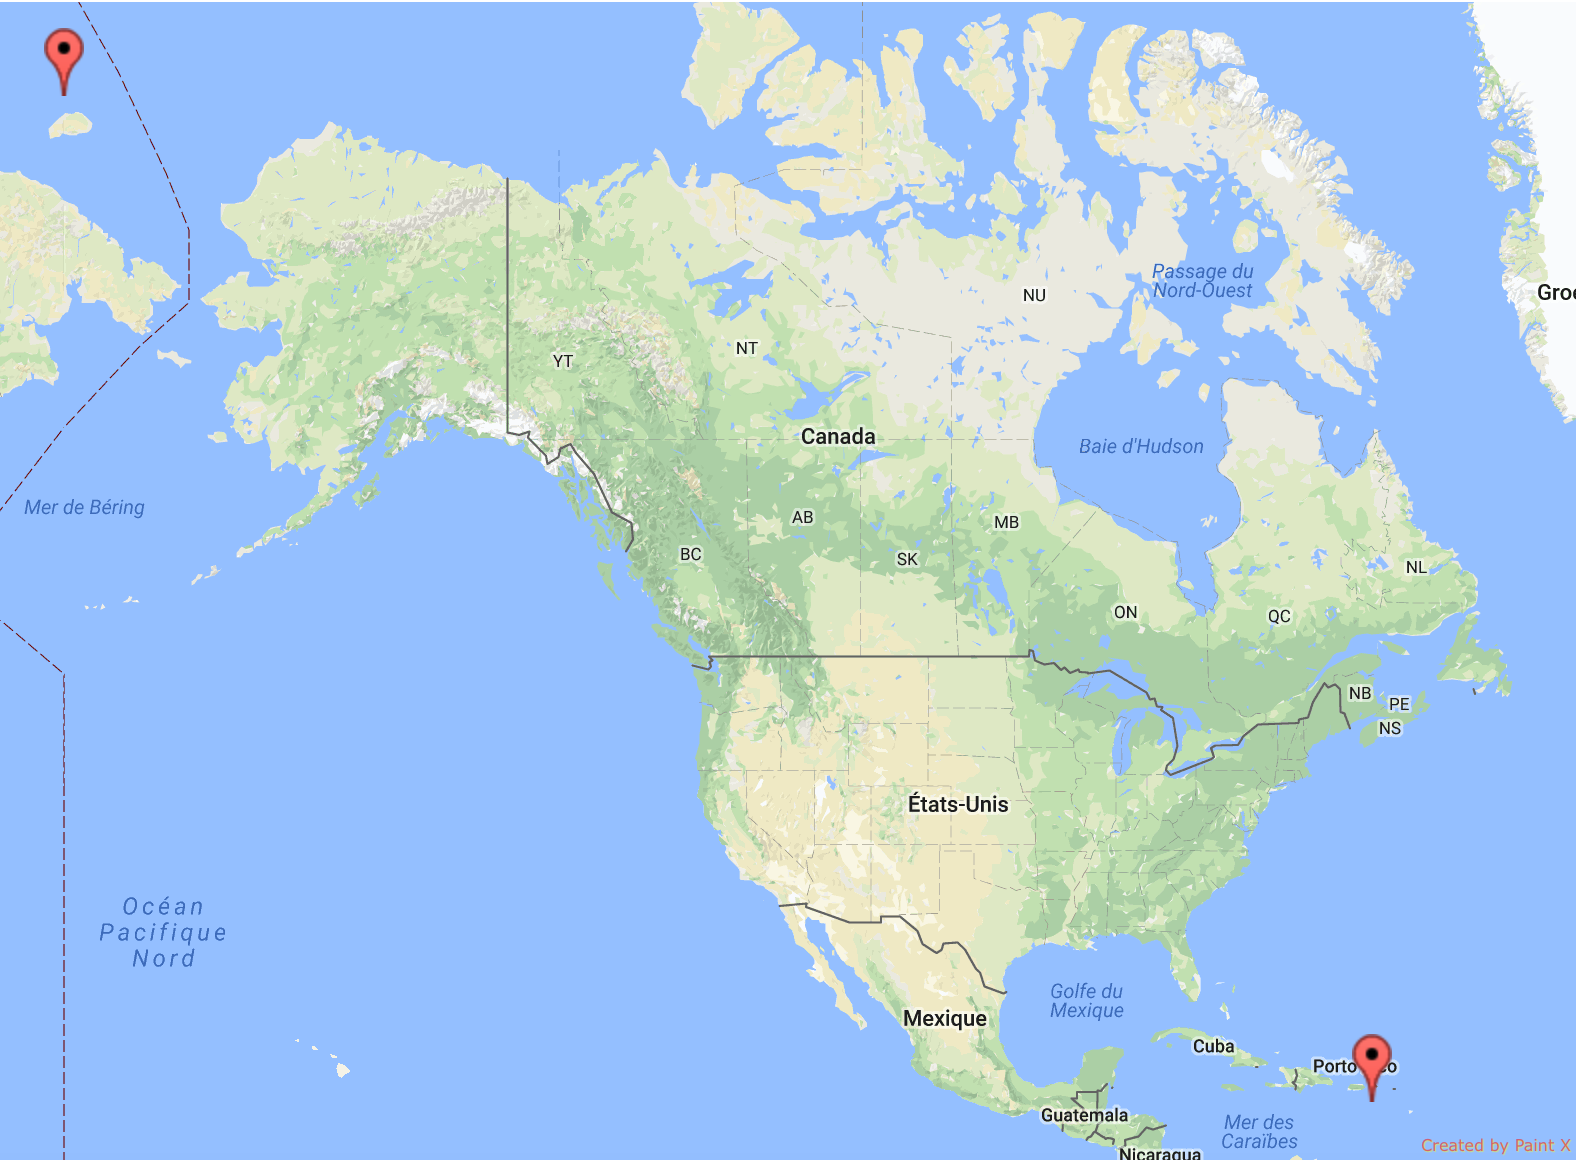
\includegraphics[scale=0.15]{map.png}
\end{figure}

As we are interested in estimating the population in the United States, we will need to perform some preprocessing to remove areas corresponding to Canada, Mexico and other countries involved.

\item 
The second data source is satellite imagery captured by Landsat 7, which serves as the raw input for our neural network. This data is available on several websites but we will extract it through the Google Earth Engine API.  The images will be chosen to align perfectly with (a perhaps coarsened) grid defined by the census data. We will randomly sort these images into training and validation sets.

The images we consider are approximately $5\mathrm{km}\times 5 \mathrm{km}$. To clarify what this means, suppose that $1^\circ$ in latitude and $2^\circ$ in longitude are respectively the best approximations to 5km in real distance. Then we will choose data from the population grid
and satellite images so that they cover exactly $1^\circ$ in latitude and $2^\circ$ in longitude.
\end{enumerate}
\vspace{-0.5cm}
\part*{The Problem}
\noindent As mentioned above, we will approach this task as a classification problem. Based on the area captured on a single image, we will determine the optimal number of classes and their precise definition. 

Using the census data as labels, we will then use a pre-trained convolutional neural network (Vgg16) to obtain a classifier. Once the CNN is trained, we will evaluate it on our holdout set of satellite images. The precise metric to measure the performance is yet to be determined but we will use tools studied in this course. In this phase, we will determine the optimal number of epochs and the value of other relevant hyperparameters. We expect this to be a difficult step that will require a considerable amount of time and effort. \vspace{-0.5cm}

\part*{Scope of the project}
Initially, the scope of the project is restricted to the continental United States. However, if the continental US turns out to be a rather ambitious task, we would consider limiting our scope to neighboring states such as Colorado and Ohio which happen to be almost perfectly rectangular (In fact, Colorado is exactly rectangular). We expect this to be a simplified setting as in this case we would study states that have the same architectural and urban patterns and therefore train the CNN quite efficiently.

\part*{Application of the project}

It is crucial problem for every government to accurately estimate the geographical distribution of their countries’ population. For example, local governments and cities often receive funding based on the population of their jurisdiction. In the absence of further data, the government has limited access to this information in between two census years. Intricate mathematical models are frequently used to predict the evolution of the population, however, there is often little opportunity to validate these predictions. Our project might give an answer to this problem (if it performs well) by allowing us to predict the population of a given geographical area in an inexpensive way. 

Another use of this project would be related to intelligence agencies allowing them to assess a country’s population even though, as in the case of North Korea, some countries keep this information secret or often falsify it. 

\end{document}



\bibliographystyle{Martin}
\bibliography{citations}


\end{document}
% vim: set spelllang=en_gb:
% DO NOT EDIT THIS LINE: $Id: 5a82d48375050ad241226f53d925effecdfdfb22 $
